\documentclass[12pt]{letter}
\usepackage{amsmath,amsfonts,amsthm,amstext,amssymb,graphicx, multicol,fancyhdr,lastpage,fullpage,framed,fancybox,enumerate,tikz,color,mathrsfs, polynom, pifont, stmaryrd}
\usepackage[margin=0.6in,headsep=3pt, headheight=15pt]{geometry}

% ----------------------------------------------------------
% Custom Definitions, Commands, Environments, etc.

% Sets of numbers
\def\R{\mathbb{R}} % The reals
\def\N{\mathbb{N}} % The naturals
\def\Z{\mathbb{Z}} % The integers
\def\Q{\mathbb{Q}} % The rationals
\def\C{\mathbb{C}} % The complex
\def\F{\mathbb{F}} % Field

% Blank space
\newcommand{\blank}[1]{\underline{\hspace{#1}}} % Blank space

% Change font colors
\newcommand{\cyan}[1]{{\color{cyan}{#1}}} % Changes font to cyan
\newcommand{\red}[1]{{\color{red}{#1}}} % Changes font to red
\newcommand{\magenta}[1]{{\color{magenta}{#1}}} % Changes font to magenta
\newcommand{\orange}[1]{{\color{orange}{#1}}} % Changes font to orange
\newcommand{\yellow}[1]{{\color{yellow}{#1}}} % Changes font to yellow
\newcommand{\violet}[1]{{\color{violet}{#1}}} % Changes font to violet
\newcommand{\green}[1]{{\color{green}{#1}}} % Changes font to green
\newcommand{\blue}[1]{{\color{blue}{#1}}} % Changes font to blue
\newcommand{\white}[1]{{\color{white}{#1}}} % Changes font to white

% Fitted inclusion symbols
\newcommand{\fp}[1]{\left({#1}\right)} % Fitted parentheses around content
\newcommand{\fb}[1]{\left[{#1}\right]} % Fitted brackets
\newcommand{\lhoi}[1]{\left({#1}\right]} % Left half-open interval
\newcommand{\rhoi}[1]{\left[{#1}\right)} % Right half-open interval
\newcommand{\set}[1]{\left\{{#1}\right\}} % Fitted braces (useful for sets)
\newcommand{\av}[1]{\left|{#1}\right|} % Fitted absolute value bars
\newcommand{\step}[1]{\left\llbracket {#1} \right\rrbracket}

% Augmented Matrix Environment
\newenvironment{amatrix}[1]{%
	\left[\begin{array}{@{}*{#1}{c}|c@{}}
	}{%
	\end{array}\right]
}

% Miscellaneous
\def\then{\Rightarrow}
\def\to{\rightarrow}
\def\d{^{\circ}}
\newcommand{\?}{\stackrel{?}{=}}
\newcommand{\cmark}{\text{ \ding{51}}}
\newcommand{\xmark}{\text{ \ding{55}}}



% Coordinate Plane (Four-Quadrant)
\def\coordplane {
	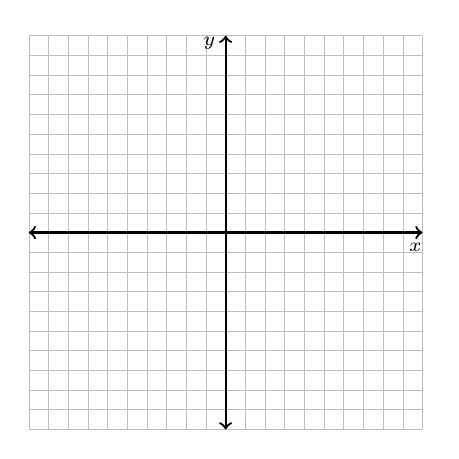
\begin{tikzpicture}        \draw[step=0.25cm,black,very thin,opacity=0.25] (-2.5cm, -2.5cm) grid (2.5cm, 2.5cm);
	\draw[<->,thick,black] (-2.5cm, 0) -- (2.5cm, 0) node[anchor=north west,pos=0.94,font=\scriptsize]{$x$};
	\draw[<->,thick,black] (0,-2.5cm) -- (0, 2.5cm) node[anchor=south east,font=\scriptsize,pos=0.94]{$y$};
	\end{tikzpicture}
}

% Coordinate Plane (One-Quadrant)
\def\onequad {
	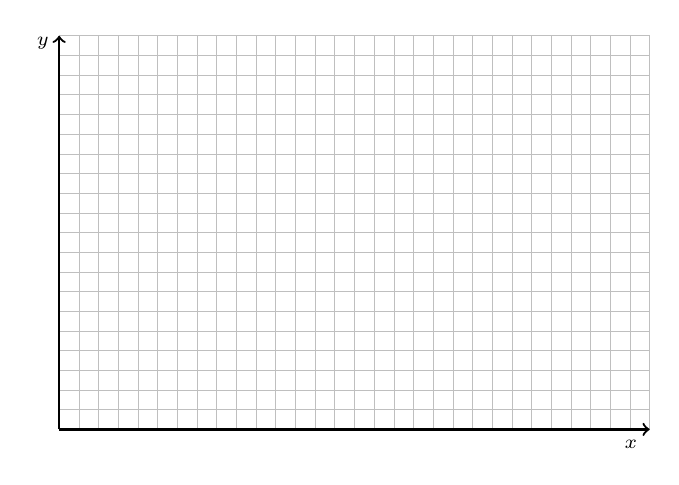
\begin{tikzpicture}
	\draw[step=0.25cm, black, very thin, opacity=0.25] (0,0) grid (7.5cm,5cm);
	\draw[->, thick, black] (0,0) -- (7.5cm, 0) node[anchor=north west,font=\scriptsize,pos=0.94]{$x$};
	\draw[->, black, thick] (0,0) -- (0,5cm) node[anchor=south east,font=\scriptsize,pos=0.94]{$y$};
	\end{tikzpicture}
}

% Counters
\newcounter{exercise}

% Exercise environment (auto-numbered)
\newenvironment{exercise}[1][]{\begin{framed}\refstepcounter{exercise}\textbf{Exercise~\theexercise:} #1}{\end{framed}}

% Book exercise environment
\newenvironment{bex}[2] {
	\begin{framed}
		\textbf{Book Exercise {#1}:} #2
	\end{framed}	
}
% ----------------------------------------------------------

% ----------------------------------------------------------
% Header and Footer Information
% \pagestyle{fancy}
% \fancyhf{}
% \renewcommand{\headrulewidth}{0pt}
% \rhead{Name: \blank{2in}}
% \lhead{@}
% \rfoot{Page \thepage \, of \,\pageref{LastPage}}
% ----------------------------------------------------------
\author{Jacob Ayers}

\begin{document}
	
	\begin{center}
		\textbf{MAT 130 \\ Final Grade Calculation Examples}
	\end{center}
	
	\textbf{\textit{Example 1}} \\
	Suppose a student earns the following scores on the course's assignments:
	
	\begin{tabular}{|c|c|c|} \hline
		\textbf{Assignment} & \textbf{Category} & \textbf{Grade} \\ \hline
		Assignment 1 & Assignments & 95 \\ \hline
		Assignment 2 & Assignments & 88 \\ \hline
		Assignment 3 & Assignments & 91 \\ \hline
		Assignment 4 & Assignments & 73 \\ \hline
		Assignment 5 & Assignments & 84 \\ \hline
		Assignment 6 & Assignments & 86 \\ \hline
		Assignment 7 & Assignments & 100 \\ \hline
		Assignment 8 & Assignments & 79 \\ \hline
		Assignment 9 & Assignments & 85 \\ \hline
		Assignment 10 & Assignments & 69 \\ \hline
		Assignment 11 & Assignments & 78 \\ \hline
		Assignment 12 & Assignments & 92 \\ \hline
		Exam 1 & Midterm Exams & 80 \\ \hline
		Exam 2 & Midterm Exams & 84 \\ \hline
		Final Exam & Final Exam & 77 \\ \hline
	\end{tabular}

	\textit{Component 1: Assignments} \\
	The two lowest scores (69 and 73) are dropped from the calculation. The student's average grade on assignments is $$\dfrac{95 + 88 + 91 + 84 + 86 + 100 + 79 + 85 + 78 + 92}{1000} = 0.878$$
	
	\textit{Component 2: Midterm Exams} \\
	The student's average grade on midterm exams is $$\dfrac{80 + 84}{200} = 0.82$$
	
	\textit{Component 3: Final Exam} \\
	No calculation necessary -- the student's final exam grade is 77\% ($0.77$).
	
	\textit{Final Grade} \\
	Remember, the weights for each category are as follows: \begin{itemize}
		\item Assignments: 20\%
		\item Midterm Exams: 60\%
		\item Final Exam: 20\%
	\end{itemize}
	So the student's final grade is $$0.878(20) + 0.82(60) + 0.77(20) = 82.16\%$$ which is a B.
	
	\newpage
	
	\textbf{\textit{Example 2}} \\
	Another student earns the following scores on the course's assignments:
	
	\begin{tabular}{|c|c|c|} \hline
		\textbf{Assignment} & \textbf{Category} & \textbf{Grade} \\ \hline
		Assignment 1 & Assignments & 82 \\ \hline
		Assignment 2 & Assignments & 76 \\ \hline
		Assignment 3 & Assignments & 77 \\ \hline
		Assignment 4 & Assignments & 80 \\ \hline
		Assignment 5 & Assignments & 87 \\ \hline
		Assignment 6 & Assignments & 70 \\ \hline
		Assignment 7 & Assignments & 75 \\ \hline
		Assignment 8 & Assignments & 91 \\ \hline
		Assignment 9 & Assignments & 0 \\ \hline
		Assignment 10 & Assignments & 81 \\ \hline
		Assignment 11 & Assignments & 86 \\ \hline
		Assignment 12 & Assignments & 72 \\ \hline
		Exam 1 & Midterm Exams & 68 \\ \hline
		Exam 2 & Midterm Exams & 72 \\ \hline
		Final Exam & Final Exam & 85 \\ \hline
	\end{tabular}
	
	\textit{Component 1: Assignments} \\
	The two lowest scores (0 and 70) are dropped from the calculation. The student's average grade on assignments is $$\dfrac{82 + 76 + 77 + 80 + 87 + 75 + 91 + 81 + 86 + 72}{1000} = 0.807$$
	
	\textit{Component 2: Midterm Exams} \\
	The student's average grade on midterm exams is $$\dfrac{68 + 72}{200} = 0.7$$
	
	\textit{Component 3: Final Exam} \\
	No calculation necessary -- the student's final exam grade is 85\% ($0.85$).
	
	\textit{Final Grade} \\
	Using the same weights as before, the student's final grade is $$0.807(20) + 0.7(60) + 0.85(20) = 75.14\%$$ which is a C.
	
	\newpage
	
	
\end{document}